% Opsætter KU Tex dokument
%%%%%%%%%%%%%%%%%%%%%%%%%%%%%%%%%%%%%%%%%%%%%%%%%%%%%%%%%%%%%%%%%%%%%%%%%%%%%%%%
\documentclass{article}                                                        %
\usepackage[a4paper, hmargin={2.8cm, 2.8cm}, vmargin={2.5cm, 2.5cm}]{geometry} %
\usepackage{eso-pic}  % \AddToShipoutPicture                                   %
\usepackage{graphicx} % \includegraphics                                       %
\usepackage{subfig}    
\usepackage{setspace}                                                        %
%%%%%%%%%%%%%%%%%%%%%%%%%%%%%%%%%%%%%%%%%%%%%%%%%%%%%%%%%%%%%%%%%%%%%%%%%%%%%%%%

% Pakker til skrifttyper, tekst osv.
%%%%%%%%%%%%%%%%%%%%%%%%%%%%%%%%%%%%%%%%%%%%%%%%%%%%%%%%%%%%%%%%%%%%%%%%%%%%%%%%
    \usepackage[utf8]{inputenc}  % Implementere Unicode                        %
    \usepackage[T1]{fontenc}     % Unicode skrifttype fx. é skrives som 1 tegn %
    %\usepackage[danish]{babel}   % Dansk Ordbog                                %
    \usepackage{microtype}       % Forbedre linjeombrydningen                  %
    \usepackage{libertine}       % Skrifttype                                  %
%%%%%%%%%%%%%%%%%%%%%%%%%%%%%%%%%%%%%%%%%%%%%%%%%%%%%%%%%%%%%%%%%%%%%%%%%%%%%%%%

% Pakker til matematik og kode.
%%%%%%%%%%%%%%%%%%%%%%%%%%%%%%%%%%%%%%%%%%%%%%%%%%%%%%%%%%%%%%%%%%%%%%%%%%%%%%%%
    \usepackage{mathtools}       % Udvidelse til amsmath pakken                %
    \usepackage{amsthm}          % Pakke til bevisførelse                      %
    \usepackage{amssymb}         % Extra matematiske symboler                  %				
	\usepackage{mychemistry}												   %
	\usepackage[version=3]{mhchem}											   %
	\usepackage{wrapfig}													   %
	\usepackage{siunitx}	
	\usepackage{anyfontsize}
	\usepackage{url}
	\usepackage{ragged2e}
	\usepackage{algorithm2e}
	\usepackage[final]{pdfpages}
	\usepackage{listings}
	\usepackage{tikz}
	\usepackage{multirow}
	\usepackage{makecell}
	\usepackage{fourier} 
	\usepackage{array}
	\usepackage{todonotes}
	\usepackage{pdflscape}
	\usetikzlibrary{arrows,shapes}
	\usepackage{titlesec}
	\usepackage{hyperref}
	\usepackage{url}
	\usepackage[nottoc,numbib]{tocbibind}
	
	\urlstyle{same}
	\tikzstyle{vertex}=[circle,fill=white!25,minimum size=20pt,inner sep=0pt]
	\tikzstyle{edge} = [draw,thick,-]

	\definecolor{light-gray}{gray}{0.85}
	\definecolor{dkgreen}{RGB}{0.0,128.0,43.0}
	\lstdefinelanguage{FSharp}%
{morekeywords={new, match, with, rec, open, module, namespace, type, of, member, % 
and, for, while, true, false, in, do, begin, fun, function, return, yield, try, %end
mutable, if, then, else, cloud, async, static, use, abstract, interface, inherit, finally, int },
  otherkeywords={ let!, return!, do!, yield!, use!, var, from, select, where, order, by },
  keywordstyle=\color{bluekeywords},
  sensitive=true,
  basicstyle=\ttfamily,
	breaklines=true,
  xleftmargin=\parindent,
  aboveskip=\bigskipamount,
	tabsize=4,
  morecomment=[l][\color{dkgreen}]{///},
  morecomment=[l][\color{dkgreen}]{//},
  morecomment=[l][\color{dkgreen}]{(*},
  morecomment=[s][\color{dkgreen}]{},
  morestring=[b]",
  showstringspaces=false,
  literate={`}{\`}1,
  stringstyle=\color{redstrings},
}
	
	\lstset{frame=tb,
  	language=[sharp]C,			%CHANGE LANGUAGE
  	aboveskip=3mm,
  	belowskip=3mm,
  	showstringspaces=false,
  	columns=flexible,
  	basicstyle={\small\ttfamily},
  	numbers=none,
  	numberstyle=\tiny\color{gray},
  	keywordstyle=\color{blue},
  	commentstyle=\color{dkgreen},
  	stringstyle=\color{red},
  	breaklines=true,
  	breakatwhitespace=true,
  	tabsize=3,
  	backgroundcolor=\color{light-gray},
	}
												   %
%%%%%%%%%%%%%%%%%%%%%%%%%%%%%%%%%%%%%%%%%%%%%%%%%%%%%%%%%%%%%%%%%%%%%%%%%%%%%%%%

% Pakker til layout.
%%%%%%%%%%%%%%%%%%%%%%%%%%%%%%%%%%%%%%%%%%%%%%%%%%%%%%%%%%%%%%%%%%%%%%%%%%%%%%%%
    \usepackage{fancyhdr}            % Gør det muligt at bruge sidehoveder     %
    \usepackage{graphicx}            % Mulighed for bl.a. \includegraphics     %
    \usepackage{colortbl}            % Hvis man vil farvelægge sine tabeller   %
    \usepackage{array}               % Gør miljøerne array og tabular bedre    %
    \usepackage{parskip}             % Første paragraf i afsnit indrykkes ikke %
    \usepackage{titlesec}            % Tilpassing af afstand mellem sektioner  %
    \usepackage[lastpage,user]{zref} % Side x af y                             %
%%%%%%%%%%%%%%%%%%%%%%%%%%%%%%%%%%%%%%%%%%%%%%%%%%%%%%%%%%%%%%%%%%%%%%%%%%%%%%%%


% Implementerer en række makroer og de pakker der er importeret
%%%%%%%%%%%%%%%%%%%%%%%%%%%%%%%%%%%%%%%%%%%%%%%%%%%%%%%%%%%%%%%%%%%%%%%%%%%%%%%%
    \pagestyle{fancy}                        % Implementerer sidehoved         %
    \lhead{University of Copenhagen}                % Venstre sidehoved               %
    \rhead{Casper Bresdahl, Karl Levinsen}                             % Højre sidehoved      %
    \cfoot{\thepage\ of \zpageref{LastPage}} % Side x af y                     %
    \newtheorem*{prp}{Propostion}            % Skaber nyt theorem  
    \renewcommand{\baselinestretch}{1.5}       %
%%%%%%%%%%%%%%%%%%%%%%%%%%%%%%%%%%%%%%%%%%%%%%%%%%%%%%%%%%%%%%%%%%%%%%%%%%%%%%%%

% Mindsker afstanden mellem sektioner
%%%%%%%%%%%%%%%%%%%%%%%%%%%%%%%%%%%%%%%%%%%%%%%%%%%%%%%%%%%%%%%%%%%%%%%%%%%%%%%%%%
\titlespacing\section{0pt}{12pt plus 4pt minus 2pt}{0pt plus 1pt minus 3pt}      %
\titlespacing\subsection{0pt}{12pt plus 4pt minus 2pt}{0pt plus 1pt minus 3pt}   %
\titlespacing\subsubsection{0pt}{12pt plus 4pt minus 2pt}{0pt plus 1pt minus 3pt}%
%%%%%%%%%%%%%%%%%%%%%%%%%%%%%%%%%%%%%%%%%%%%%%%%%%%%%%%%%%%%%%%%%%%%%%%%%%%%%%%%%%

%Ændrer størelsen på sections
%%%%%%%%%%%%%%%%%%%%%%%%%%%%%%%%%%%%%%%%%%%%%%%%%%%%%%%%%%%%%%%%%%%%%%%%%%%%%%%%%%
\titleformat{\section}
{\normalfont\fontsize{14}{16}\bfseries}{\thesection}{1em}{}
\titleformat{\subsection}
{\normalfont\fontsize{12}{14}\bfseries}{\thesubsection}{1em}{}
\titleformat{\subsubsection}
{\normalfont\fontsize{11}{13}\bfseries}{\thesubsubsection}{1em}{}
%%%%%%%%%%%%%%%%%%%%%%%%%%%%%%%%%%%%%%%%%%%%%%%%%%%%%%%%%%%%%%%%%%%%%%%%%%%%%%%%%%

%%%%%%%%%%%%
% Document %
%%%%%%%%%%%%

\begin{document}

\begin{titlepage}

\newcommand{\HRule}{\rule{\linewidth}{0.5mm}} % Defines a new command for the horizontal lines, change thickness here

\begin{center}
 % Center everything on the page
 
%----------------------------------------------------------------------------------------
%	HEADING SECTIONS
%----------------------------------------------------------------------------------------

\textsc{\LARGE University of Copenhagen}\\[1.5cm] % Name of your university/college
\textsc{\Large Computer Science}\\[0.5cm] % Major heading such as course name
\textsc{\large Bachelor Thesis}\\[0.5cm] % Minor heading such as course title

%----------------------------------------------------------------------------------------
%	TITLE SECTION
%----------------------------------------------------------------------------------------

\HRule \\[0.4cm]
{ \huge \bfseries Synthesis of Actor Code and tests =====TBD======}\\[0.4cm] % Title of your document
\HRule \\[1.5cm]
 
%----------------------------------------------------------------------------------------
%	AUTHOR SECTION
%----------------------------------------------------------------------------------------

\begin{minipage}{0.4\textwidth}
\begin{flushleft} \large
\emph{Authors:}\\ 
% Your name
Casper \textsc{Bresdahl} \\
Karl \textsc{Levinsen}
\end{flushleft}
\end{minipage}
~
\begin{minipage}{0.4\textwidth}
\begin{flushright} \large
\emph{Supervisor:} \\
Boris \textsc{Düdder}\\
\hfill
\end{flushright}
\end{minipage}\\[2cm]

% If you don't want a supervisor, uncomment the two lines below and remove the section above
%\Large \emph{Forfattere:}\\
%Axel \textsc{Christof}\\% Your name
%Casper \textsc{Bresdahl}\\
%Emilie \textsc{Bentsen}\\[1cm] 

%----------------------------------------------------------------------------------------
%	DATE SECTION
%----------------------------------------------------------------------------------------

{\large \today}\\[2cm] % Date, change the \today to a set date if you want to be precise

%----------------------------------------------------------------------------------------
%	LOGO SECTION
%----------------------------------------------------------------------------------------


\includegraphics{logo.png}\\[1cm] % Include a department/university logo - this will require the graphicx package
 
%----------------------------------------------------------------------------------------

\vfill % Fill the rest of the page with whitespace

%Disse linjer skaber forside, evt indholdsfortegnelse, og sætter sidetal
%%%%%%%%%%%%%%%%%%%%%%%%%%%%%%%%%%%%%%%%%%%%%%%%%%%%%%%%%%%%%%%%%%%%%%%%%%%%%%%%
									                                           %
    \thispagestyle{empty}   % Fjerner sidetal forside                          %
        % Slå disse til hvis der ønskes indholdsfortegnelse                    %
        %%%%%%%%%%%%%%%%%%%%%%%%%%%%%%%%%%%%%%%%%%%%%%%%%%%%%%%%%%%%%%%%%%%%%%%% 
            \newpage                % Side til indholdsfortegnelse            %
            \thispagestyle{empty}   % Fjerner sidetal fra indholdsfortegnelse %
            \tableofcontents        % Skaber indholdsfortegnelse              %
    \end{center}
    %\section*{Forord}
    	
		
        %%%%%%%%%%%%%%%%%%%%%%%%%%%%%%%%%%%%%%%%%%%%%%%%%%%%%%%%%%%%%%%%%%%%%%%%
    \newpage                % Første rigtige side
    \setcounter{page}{1}    % Sætter rigtigt sidetal på første side
%%%%%%%%%%%%%%%%%%%%%%%%%%%%%%%%%%%%%%%%%%%%%%%%%%%%%%%%%%%%%%%%%%%%%%%%%%%%%

\end{titlepage}
{\fontsize{10}{14}\selectfont

\section{Introduction} \label{intro}
In this thesis we have extended upon a sandbox like demo project from Microsoft \cite{AdventureGame} which resembles an adventure game and is written in a distributed fashion with Orleans. We have then decomposed it into a code repository with the  purpose of using the Combinatory Logic Synthesizer, a type based tool to automatically compose larger systems from a repository of code components, to create different variations of the game based on definitions written in a metalanguage. Our goal has been to synthesize code with timers, synthesizing code where we dispose timers, synthesizing code where we create other actors and to be able to define a list of parameters in our metalanguage and then synthesize code where only the defined parameters are present in the game variation. Our goal has also been to test our application, both as the initial program as well as the combinated variations of the game. This means synthesizing tests in the same way as our code, such that a given variation has tests alongside the program specific to that variation. 
\todo{Extend introduction to introduce testing?}\\
We will begin by looking at the theory behind the actor model and Orleans, then we will move to the theory of the Combinatory Logic Synthesizer and how it works. After that we will look into more detail about the extensions we have made to the Microsoft project. We will then look into the design decisions about decomposing the code, the issues we faced and what improvements we could have made. We will also look into what makes a good component and ask ourselves if we have achieved good decomposition. 
Then we will look into the relevant theory of testing software, followed by a deeper dive into our testing, meaning the tests themselves alongside the tests as combinators in the CLS. We will be discussing our implementation and looking at some of the obstacles we faced during our process of creating tests\todo{Change for a more comprehensive description}. We will then comment on our results and lastly make our conclusions.
\begin{itemize}
	\item Abstract
	\item Introduction
	\item Actor model - 4
	\item CLS - 4
	\item Our product - 4
	\item Discussion of implementation - 12
	\item Testing theory - 4
	\item Discussion of testing - 12
	\item Results - 4
	\item Conclusion
\end{itemize}
\section{Actor model}
The actor model is a programming model utilising concurrent computation for developing parallel, distributed and mobile systems. An actor can do three things: it can send messages to other actors, it can update its local state or it can create more actors. All actors work concurrently and asynchronously together by sending and receiving messages. When an actor receives a message it performs some specified task based on its local state and the content of the received message. This task can be to perform some computation, and the result can then be passed along to another actor in a new message \cite{ActorModelPaper}.\\
All actors have a globally unique name which is used to determine to which actor a message is sent. Name of actors may be communicated in messages such that an actor knows who to send the next message to, or such that an actor knows who just sent it a message. An actor's state is local and can not be shared with other actors, and thus, to change the behaviour of an actor, another actor must send a message specifying it to change state. The path a message takes and what network delays a message may encounter is not specified and thus messages may arrive out of order \cite{ActorModelPaper}.\\
\begin{figure}[H]
	\centering
	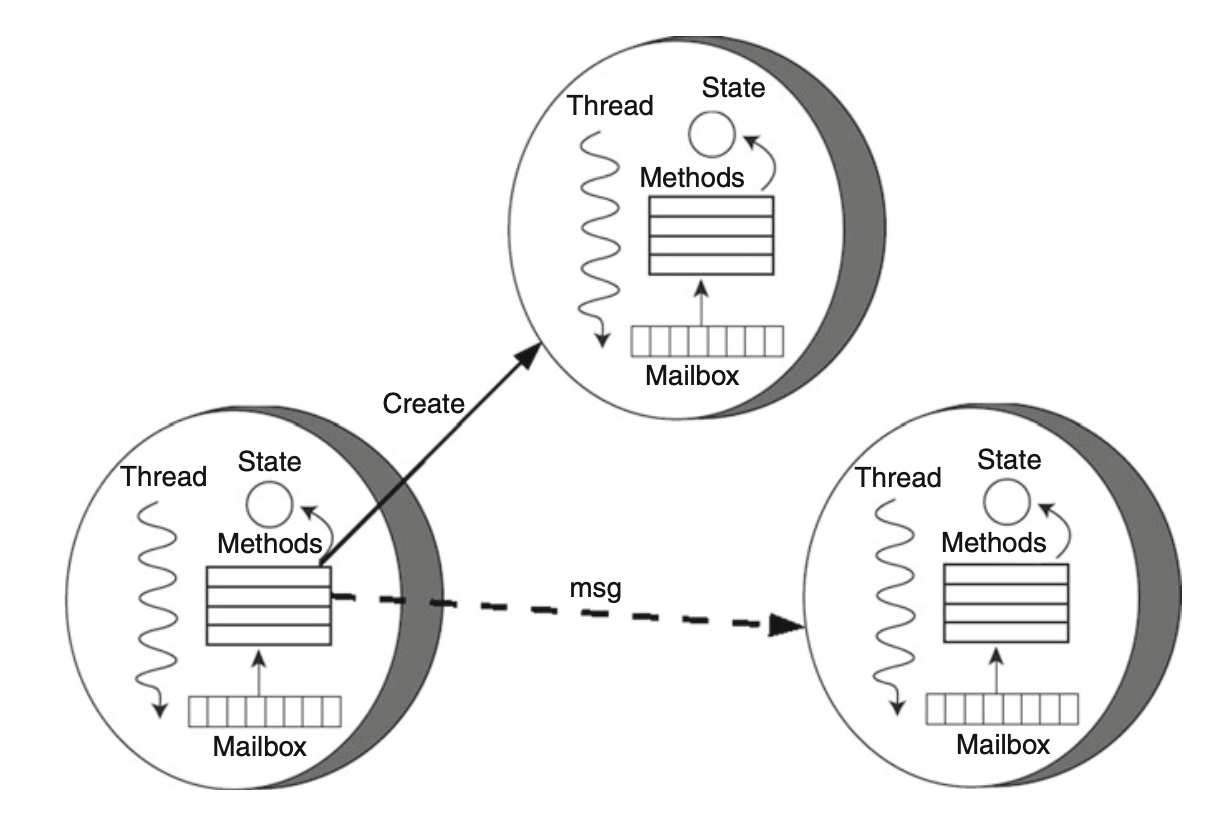
\includegraphics[width=0.85\linewidth]{Materials/ActorModel/AMDemonstrated}
	\caption{An actor consists of methods, a mailbox for queued messages and a local state. Actors can send messages, change state based on a received message and create other actors. Figures is from \cite{ActorModelPaper}.}
	\label{AMDemonstrated}
\end{figure}
As seen in \autoref{AMDemonstrated} an actor can be illustrated as an entity with a mailbox, a set of methods and a local state. The mailbox is often implemented as a queue \cite{ActorModelPaper}, and is used to store messages which arrive while the actor is already handling another message. The methods may make the actor change its state, make the actor create a new actor or send a message to another actor.\\
As already hinted at above, the core semantic properties of an actor are \textit{encapsulation} of the local state, the ability to \textit{atomically} execute methods, \textit{fairness} in scheduling actors and \textit{location transparency} to enable distributed execution and mobility \cite{ActorModelPaper}, and all of these we will look into next.
 
\subsubsection{Encapsulation and Atomicity}
Encapsulation means each actor has its own state, and thus all changes to the state of an actor has to come in a message sent from another actor. The notion of encapsulation is also one of the corner stones of object oriented programming where each object also has its own state. This can be very useful to enforce an object oriented decomposition in code, and may make actors look a lot like objects \cite{ActorModelPaper}.\\
Encapsulation has also lead to the notion of atomicity. In a sequential program one object may call a method in another object. This method will then run to the end before another object can call the method again. The called object may or may not have changed state during the method call, but we can only reason about this because the method call can not be interrupted by another method call. Because all method calls are run uninterrupted, we can reason about the object's behaviour given we know its state prior to the method call \cite{ActorModelPaper}.\\
In a concurrent setting an object may call a method in another object, but right after a third object does the same. If the first method call would be interrupted to accommodate the second, the object's state might already be altered, and we can no longer reason about the behaviour the object exhibits after a call to its method. This would lead to inconsistencies in the system as these concurrent calls can happen at any time. To guarantee we can reason about object behaviour in actors we therefore must guarantee that received messaged are handled atomically, meaning that the processing of a message happens in one step, and is not interrupted by new messages. This ensures that the encapsulated state is consistent throughout the execution of a program \cite{ActorModelPaper}.

\subsubsection{Fairness}
The notion of fairness states that all actors are scheduled time to run, and that they will make progress given they have computations to do. It also states that all messages are guaranteed to reach their destination unless that actor has been permanently disabled. The notion of fairness allows us to reason about the liveness properties of actor programs \cite{ActorModelPaper}. Here we note that an actor program is started by an external message sent to an actor, and that an actor program terminates when all actors are idle and no external message can be passed to any actors. An actor is considered idle if it has no pending messages in its mailbox.

\subsubsection{Location transparency}
Location transparency provides an abstraction for the programmers who need to make actors communicate. In the actor model the location of actors does not determine its name. Two actors might run on the same computer in the same core, or they might run on two different machines in two different countries. Location transparent naming enables the programmers no to worry about the actors physical location. \cite{ActorModelPaper}.\\
Mobility is defined as the ability for a computation to migrate to another node \cite{ActorModelPaper}. This is important for load-balancing, fault-tolerance, and reconfiguration, and is useful in achieving scalable performance \cite{ActorModelPaper} as an actor lifting a lot of heavy work along other actors doing the same on the same machine can seamlessly be moved to another machine in an attempt to alleviate the workload on that machine.

\subsubsection{Synchronization}
\begin{figure}[H]
	\centering
	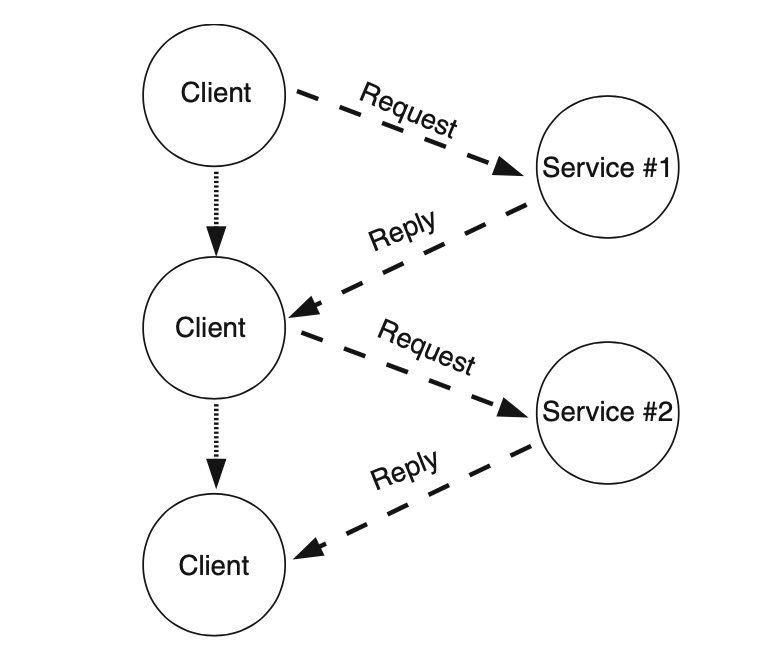
\includegraphics[width=0.6\linewidth]{Materials/ActorModel/AMCommunication}
	\caption{An illustration of how RPC like communication works. Figures is from \cite{ActorModelPaper}.}
	\label{AMCommunication}
\end{figure}
One way to achieve synchronization of actors is through Remote Procedure Call like message passing (RPC), which is a common communication pattern in actor systems \cite{ActorModelPaper}. In a situation where an actor wants to make sure another actor has received its message before it communicates it to others or where the order of messages matter RPC like messaging is a big help. In RPC like communication the sender of a message waits for a reply before it continues to process other messages. An actor might want to wait for a reply if it needs the information in the reply to continue its computation. This can be seen in \autoref{AMCommunication} where the client sends a message to a service and waits for the reply before sending another message to another service \cite{ActorModelPaper}.\\

\subsection{Orleans}
Orleans is a framework for C\# developed by Microsoft. The framework simplifies several aspects of the actor model to make it a lot easier for programmers to write actor based code. Some of the simplifications Orleans helps with are lifecycle management of actors in the application code, to deal with distributed race conditions, to handle failures and recovery of actors after server crashes, and to make an abstraction for actor placement.\\
An important abstraction the developers of Orleans have made is the notion of virtual actors. In Orleans we work with virtual actors which are based on the actors described previously, but they implement some important differences which abstract away some of the more cumbersome implementations of actors. The first of these is perpetual existence which states that virtual actors are logical entities which always exists. A virtual actor can not explicitly be created or destroyed. Its existence is unaffected by the server which runs it, and thus also unaffected by the server crashing. Given that a virtual actor always exists, it is also always addressable \cite{OrleansPaper}.\\
Another great help Orleans implement is automatic instantiation. The Orleans' runtime automatically creates instantiations of actors called activations. An actor can only be instantiated if it has a request pending. When a request is sent to an actor the Orleans runtime automatically instantiates an activation on a server. If the server should later crash, the Orleans runtime automatically re-instantiates the actor when the next request to it arrives. This means that the programmer does not have to program actor lifecycles themselves, but can rely on Orleans to automatically figuring out where and when to instantiate an actor. Likewise, the Orleans runtime also automatically disposes unused actors if they have been idle for a long time \cite{OrleansPaper}.\\
Orleans also takes care of the location transparency abstraction. An application running inside an actor, or communicating with an actor does not know its physical location, and neither does it need to, as long as it knows the actors name it can send it a message. Orleans allow programmers to name actors much like one would name an object in an ordinary object-oriented program.\\
Orleans allows for timers which, as the name suggests, specify code that will be run later. A timer is automatically disposed if an actor is recycled by runtime, but can otherwise be specified to fire in even intervals. Because timers 'run in the background' it is important that the programmer makes sure they are disposed when no longer needed.\\
Orleans allows actors to synchronize through RPC-like message passing as discussed in subsection '\nameref{Synchronization}'. This is done by awaiting a response from another actor. Due to atomicity the actor can not progress its method while awaiting a response. Therefore other actors or other tasks are run in the mean time while the actor waits. When the response arrives the actor will then continue the method from where it left off.
\section{Testing Theory}
%Integration
%State testing?
Testing is a quality-improvement activity meant for detecting errors in the software you write, meaning error detection, however it may sometimes falsely be referred to as "debugging" \cite{TestingCodeComplete}. Testing is a large topic, that spans way beyond testing during development, meaning it may be in place to specify our scope of testing. \\
We will look and describe the two testing areas that we have performed. While software is tested in a number of ways, we will solely look at unit testing and integration testing. \\%meh
Unit testing is the testing of a single routine, class or small program, in isolation from the rest of the system. This is to ensure that the individual classes and their methods work as intended, without any dependencies\cite{TestingCodeComplete}.
Integration, on the other hand, is testing of two or more routines, classes, etc. After unit testing, we know the individual classes or components work in isolation. Integration testing is the testing of the connection and interaction between the classes, such that we ensure the system works in unison. \\
Unit testing is performed before the integration tests, as to ensure the individual classes work, before testing them all together. If we used integration test first, and a given test failed, we would not know whether the fault was in a specific method or the communication between classes. \\
\subsection{White-box and Black-box Testing}
%basis testing
%control flow
%data flow
%AAA
We usually split testing up into two categories: black-box and white-box testing. Black-box testing refers to tests in which the tester does not have access to the source code and must hence test based on the specifications of the given methods, meaning testing based on what the method is supposed to do, hence the method works as a black-box. White-box testing is the other scenario, where the tester has access to the method. This means that the tester is aware of the control flow and routes the method can take, such that testing can rely on the inner workings of the method instead of only the specifications\cite{TestingCodeComplete}. \\
However, even though we are the developers, we do not have direct access to the code. This is because, while we do have access to the combinators and the pre-synthesised code, we will not be able to see the synthesised code doing our synthesising of our tests as well \todo{Needs rephrasing}. The synthesised code will work as a sort of black-box, since we do not actually know how the code looks like and hence making white-box testing would prove difficult, without analysing our generated files. So with this in mind, we have chosen to focus on black-box testing, as this seems as the more accessible and appropriate path to take. \\
Black-box testing is mainly split up in two parts: Data testing and state testing. Here, data testing refers to the data, meaning the input, while state testing is about the program, that is the flow, transitions, logic, and so on\cite{TestingBlackbox}. Let us look at these two parts more closely, some of the methods to use in these cases\todo{Needs rephrasing}. The two major methods under we will look at are equivalence partitioning and boundary conditions. \todo{Maybe rephrasing?}.
\subsubsection{Equivalence Partitioning}
The most important task when it comes to testing is selecting the right test cases\cite{TestingBlackbox}. After all, if we had a simple program that took an integer as input, we could, theoretically, make infinitely many tests for this. This is where equivalence partitioning, also called equivalence classing, comes in. The idea here is that we reduce the infinite possible sets of test case, while still being as effective. We want to split the data into partitions, such that we can use a single test that counts for a range of possible input. For instance, how different would it be to test for 1, 2 and 3 as input as opposed int.MaxValue? We would expect that the first three cases would act similarly, while the program would have to handle the maximum integer value differently. However, how do we know for sure what input to put in the different partitions? The short answer is we do not. Equivalence partitioning can be subjective, such that different testers may come up with different partition sets\cite{TestingBlackbox}. \todo{mere? edge cases?}
\subsubsection{Boundary Conditions}
Boundary Conditions is about testing the method at the boundaries. As a good illustration of what boundary condition is and is for, you could imagine walking along the edge of a cliff. If you can traverse this part safely, you can most likely traverse away from the edge as well. Meaning, if we can show that our methods work at the edge of their capabilities, chances are they will almost certainly work under normal conditions as well. These boundary conditions, also known as edge cases, are important since with programming, problems are more likely to occur at the edges\cite{TestingBlackbox}. This means that, for instance, if we could input any number between 1-100, it would be better to test the edges, such as 1 and 100 than numbers in the middle. \\
We can combine this with the Equivalence partitioning explained earlier. We could split our testing into two equivalence partitions. One should be the edges, those that we expect to work, meaning in our number example it could be 1 and 100. The other equivalence partition would then be outside the boundaries, meaning cases that could likely cause an error, or some unexpected behaviour. In our example, this could be 0 or -1 and 101, just outside our boundaries. 
\subsubsection{Default, Zero and Blank}
Another thing we can look at is testing our methods with a default value. In this case we mean, for instance, if our TakeDamage() method, is parsed 0, what happens then? Or the play function, which is our player's way to interact with their surroundings in the game, by entering things like "fireball witch", "go north", etc., what happens if we enter the empty string? These types of cases can be classified as forms of edge cases, but they are still important to include, as these situations may have been overlooked during implementation of the methods\cite{TestingBlackbox}.
\subsubsection{AAA}
One last thing we want to look at is the structure of the individual unit tests. Usually they conform to the AAA pattern. AAA stands for arrange, act and assert. Using this form of pattern makes it easy for other people to understand your tests\cite{TestingAdaptiveCode}. \\
The arrangement part is also referred to as the setup. Before we can actually perform a certain test, we need to set up what we need in order to carry out the tests. A simple example would be instantiation of the class to be used in the test. Without instantiating the class, we will not have a valid instance to test. \\
The act part of AAA is the execution of the method to be tested. Optimally, this should only consist of a single interaction, for instance meaning a single method call\cite{TestingCodeComplete}. This ensures that the individual tests are simple and precise. \\
The last part of AAA is the assertion. This is the actual testing part, where we will see whether our act part has performed as expected, or produced another, unforeseen, outcome. \\
\\
However, we have diverged a bit from this concept for two reasons. First off, the testing framework we are using, NUnit, allows setup code to be run from the constructor. This means that the arrange aspect can partially, if not fully, be moved to the constructor of the test class. \\
The other reason is readability and transparency. If we have a test, NUnit allows the ability to run the same code with various data input. This means we can have multiple testcases, under the same test function. At a first glance, this may look better, as there is less code in the function, however, it can make the assert part more unclear. If we want to make multiple testcases of the same test, our expected value had to be dynamic, which would obfuscate what we really intended as the expected value.\todo{Do we use this? Is it relevant?} \\
So instead, we explicitly state what the expected outcome is. 
\begin{figure} %MINDRE?
    \centering
    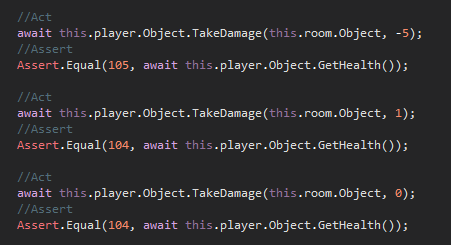
\includegraphics[width=0.8\linewidth]{Materials/TestingTheory/playerTakeDamageAAAtest}
    \caption{Part of the player's DamageTest(), showcasing the AAA structure.}
    \label{playerDamageTest}
\end{figure}
if we look at \autoref{playerDamageTest} we can see how we diverge from the described form of AAA, where our test includes the various testcases with different input, instead of feeding the data to a dynamic test. Here we can also see how we explicitly state the expected outcome for each testcase. 

% As we have been the developers of our product, we will omit black-box testing and focus on white-box testing. As stated, since white-box testing includes the source code, we can more thoroughly test our methods and hence, with white-box testing, cover the same testcases as black-box tests, making them superfluous. \\% måske?
% Now, under white-box testing we have different testing methods to make sure our tests are thorough. Futhermore, there are two aspects we will look at shortly: control-flow testing and data-flow testing. As the name suggests, control-flow testing is about testing the control statements of a method, and making sure we test all possible routes. Data-flow testing is focused on the variation of data and the idea here is that data is atleast as error-prone as control-flow and should therefore be tested as well\cite{TestingCodeComplete}. 

% \subsubsection{Structured Basis Testing}
% We will start by looking at control-flow testing. Here we have structured basis testing, which is a pretty simple concept. We want to make sure that each statement in the given method is run at least once during testing. We can use a simple approach to figuring out how many testcases are needed for basis testing at a minimum, by following these three steps\cite{TestingCodeComplete}:
% \begin{itemize}
%     \item Add a testcase for the method itself.
%     \item Add a testcase for each of the control-flow keywords in the method. (if, while, for, and, etc.)
%     \item Add a testcase for each case in a case statement. Add an additional testcase if the case statement does not include a default case.
% \end{itemize}
% For instance, if we picture a simple method that contained a simple if-statement, we would need two testcases: one for the simple path through the method, and one for the control-flow keyword if. From this we can see that, based on the complexity of the method, the number of testcases we will need to cover all statements increases quickly. \\
% So, with structured basis testing, we assure that all code of a method is executed. However, as mentioned earlier, data-flow is atleast as error-prone, and structured basis testing does not take variation of data into account.

% \subsubsection{Data-flow testing}
% With data-flow testing, we want to ensure that not only all statements are covered, but also all combinations of variables in the code. With structured basis testing, we get a weak form of data-flow testing, since this executes all lines of code, which includes all variables\cite{TestingCodeComplete}. This, in turn, gives us some of the combinations of data, but not them all. We want to extend upon the structured basis testing to include data-flow testing and this calls for more testcases. Here, we want to add all the combinations of variable states that have not been included in the structured basis testing. %Hmmmm
\subsection{Test Doubles}
%Test doubles / isolation
%Moq framework +example
The way our code is written, we have a certain focus on the room, wherein the other actors may reside. This means that a lot of the methods requires a specified room, to know where and what to look for. In short, we have high coupling between our classes. However, in unit testing, we wish to perform tests of each class in isolation, independently of the other classes. So, if we have high coupling, and yet want to test classes independently, how are we to do this? \\ This is where test doubles come in. Using test doubles, also known as scaffolding, is the means of making it easier to isolate code for testing. The point of a test double is to act as a class, including some of its functionality, so that it can be used by another class that is being tested\cite{TestingCodeComplete}. There are various test doubles available, such as fakes, dummies and mocks. Since mocking is what we are going to use, this is what we will look more into.

\subsubsection{Mocking}
The idea of mocking, or mock objects, is to mimic the behaviour of the real class we are imitating. However, we can do this in a controlled way, such that the methods of the mimicked class returns some specific values, independently of the input they receive. This means that the class will not produce any specific results based on their real implementation, but predefined output that we specify\cite{TestingAdaptiveCode}. As such, if we have a class we want to test, that is dependent on the class we mimic, we can now replace the dependency with our mimicked class. Now we have isolated the class we want to test, as all interactions with the mimic is controlled. \\
\\
To mimic the behaviour of a real class it would require us to make a new class. For each class we would like to mimic, we would have to make seperate classes for. This does not only mean that we would need a lot of extra code just for our unit tests, but also that if we were to change the actual class, we would have to change the mimic. This could, potentionally, become tedious work. To get around this, we make use of a framework, that enables us to make the mock objects dynamically, namely the Moq Framework.

\subsubsection{Moq Framework}
This will serve as a short introduction to the Moq framework and how we use it in our testing. \\
We already mentioned how making our mocked versions of the various classes manually would be tedious work. Luckily, the Moq framework makes it easy for us to mock a given class. This framework is very powerful as it allows us to manipulate the behaviour and expectations of our class\cite{TestingAdaptiveCode}. The major part of the mocking lies in the setup. When setting up a new mock, you can specify with the help of the Setup() function, what a given function should return, based on some specific or generic input. Let us take a closer look at the first line of the function body in \autoref{TakeTestMoq}. 
\begin{figure}
    \centering
    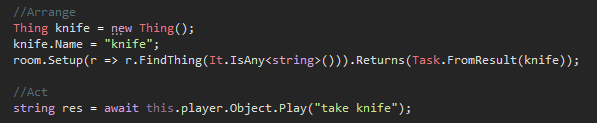
\includegraphics[width=0.9\linewidth]{Materials/TestingTheory/testTakeTestMoqExample}
    \caption{Part of player's TakeTest() showcasing the moq framework's setup}
    \label{TakeTestMoq}
\end{figure}
Here, we can see a nice example of the moq framework. The variable here, room, is of Mock<IRoomGrain>. As we can see with the lambda function, we specify that by a call to the room's FindThing() function, with an input of type string should return the newly created knife. This way, we can test the player's take command, that requires the room we are currently in, as well the items in this room, without the interaction of an actual room. This ensures that we can test the player in isolation, while also noting that the player indeed does send a message to the room grain. It should also be noted here, that while player is of type Mock<PlayerGrain>, by calling player.Object we effectively have the mocked player of type IPlayerGrain and not a player of type Mock<PlayerGrain>.

\subsubsection{Mocking a Class vs Mocking an Interface}
We would also like to shortly explain the difference between mocking a class and mocking an interface. As is made apparent in our tests, we mock both the class under testing and the classes that it depends on. The only difference in the mocking between these two is that the class under testing is a mock of the actual class, while its dependencies are mocks of their interfaces. \\
Mocking an interface creates an instance of the class that implements this interface, but with no actual implementation or logic. For instance, if we look at \autoref{TakeTestMoq}, we set the room's FindThing() function to return a knife to us. If we did not do this setup, the function would not have been implemented and given us and error instead. \todo{er det hvad den gør?} \\
Mocking a class creates an inherited class of the mocked one, which per standard uses the base implementation of their functions. So if we mock a class and make no setup, the functions will be the same. However, the smart thing about mocking these classes for testing, that function virtually the same as the original class, is that it allows us to change certain behaviour, while still maintaining the same functionality, such that we can test it properly. \todo{cite} \\
We will look more into why this is important, and how we have changed certain aspects of the code, in the DISCUSSION SECTION GRAINFACTORY. \todo{reference}

%Gem GrainFactory for discussion
% \begin{figure}
%     \centering
%     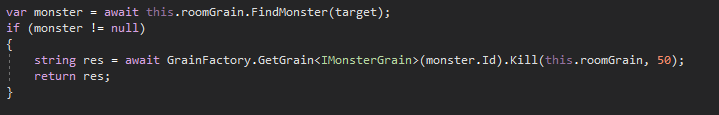
\includegraphics[width=\linewidth]{Materials/TestingTheory/FireballGrainFactory}
%     \caption{Snippet of player's Fireball() function, showcasing the problem with GrainFactory. Even if our room was mocked and returned our mocked monster's id, GrainFactory would create a real monster based on this id, as it finds no monsters with this id.}
%     \label{fireballGrainFactory}
% \end{figure}
% However, we do still have a problem, since this mocking does not cover all of our coupling of the grains. We can access different grains by calling GrainFactory.GetGrain<Type>(id), but by the nature of grains, if we call this function, with an id that does not correspond to any existing grain, it will automatically generate one for us. These methods are called inside some of the different functions of our grains, meaning that even though we can mock a monster, if a function inside player calls a function inside monster through the use of GrainFactory, it will ignore any mock monster we have created and make a real IMonsterGrain for us instead. We can see this problem illustrated in \autoref{fireballGrainFactory}. \todo{Måske cite + billede er godt til at illustrere?} So, how do we get around this? \\
% One way to side-step this issue is to mock the GrainFactory function of the class we are currently testing. To do this, we have to expose the GrainFactory function of the class, as it normally is a protected function. We would then create an override of the GrainFactory function, which means that we rewrite code in our classes due to our tests and while this is bad practice, it must be done in order to mock the GrainFactory and ensure that our grains do not make their own grains when we want them to use our mocked grains instead \todo{cite?}. \\ 
% This does open yet another issue. The new GrainFactory implementation cannot be part of our interface, such that if we want to use our mocked GrainFactory, we would use mocks of the classes instead of the interfaces (e.g. Mock<PlayerGrain> instead of Mock<IPlayerGrain>), rendering some of the interfaces functions hidden and unsuable for testing. \todo{Billeder? what to do med problemet? "maskintekst" for funktioner i vores tekst?}
\begin{thebibliography}{9}
\bibitem{ActorModelPaper}
Karmani, Rajesh K. Agha, Gul. Padua, David (ed.). 2011. 'Actors', part of 'Encyclopedia of Parallel Computing'. Springer Science+Business Media. Downloaded: November 26, 2019.

\bibitem{TestingCodeComplete}
McConnell, Steve. 2004. 'Code Complete'. Microsoft Press 2. ed. Chap. 22.

\bibitem{TestingAdaptiveCode}
Hall, Gary. 2014. 'Adaptive Code via C\#'. Microsoft Press 1. ed. Chap. 4.
\bibitem{OrleansPaper}
Bernstein, Philip A. Bykov, Sergey. Geller, Alan. et. al. 2014. 'Orleans: Distributed Virtual Actors for Programmability and Scalability'. Microsoft Research. Available at: \url{www.microsoft.com}. Downloaded: December 8, 2019.

%%%%%%%%%%%%%%%%%%%%%%%%%%%%%%%%%%%%%% SHOULD BE DELETED %%%%%%%%%%%%%%%%%%%%%%%%%%%%%%%%%%%%%%%%%%%%%%
\bibitem{book}
Marchewka, Jack T. 2015. 'Information Technology Project Management - Providing Measurable Organizational Value'. Wiley 5. ed.

\bibitem{rigsrevision}
Rigsrevisionen. 13. september 2019. 'Beretning om udvikling af det nye inddrivelsessystem og tilslutning af fordringshavere'. \url{www.rigsrevisionen.dk}. Hentet: 28. oktober 2019.

\bibitem{ugeopgave2}
Mogensen, Sten. 12. september 2019. 'Ugeopgave 2'. \url{absalon.ku.dk}. Hentet: 28. oktober 2019.

\bibitem{ugeopgave3}
Mogensen, Sten. 19. september 2019. 'Ugeopgave 3'. \url{absalon.ku.dk}. Hentet: 29. oktober 2019.

\bibitem{waterfallVsAgile}
Glowtouch.com. 'Waterfall vs. Agile: The Good, The Bad and The Misunderstood'. \url{https://www.glowtouch.com/waterfall-vs-agile-good-bad-misunderstood/}. Hentet: 29. oktober 2019.

\bibitem{scrumMaster}
Andersen, Tania. 4. januar 2018. 'Agile metoder er i dag den herskende måde at udvikle software på. Men Scrum og andre agile teknikker er ingen garanti for succes'. \url{www.version2.dk}. Hentet: 29. oktober 2019.
%%%%%%%%%%%%%%%%%%%%%%%%%%%%%%%%%%%%%% SHOULD BE DELETED %%%%%%%%%%%%%%%%%%%%%%%%%%%%%%%%%%%%%%%%%%%%%%
\end{thebibliography}

\end{document}